% This version of CVPR template is provided by Ming-Ming Cheng.
% Please leave an issue if you found a bug:
% https://github.com/MCG-NKU/CVPR_Template.

\documentclass[final]{cvpr}

\usepackage{times}
\usepackage{epsfig}
\usepackage{graphicx}
\usepackage{amsmath}
\usepackage{amssymb}

% Include other packages here, before hyperref.
\usepackage{acro}
\usepackage{csquotes}

% If you comment hyperref and then uncomment it, you should delete
% egpaper.aux before re-running latex.  (Or just hit 'q' on the first latex
% run, let it finish, and you should be clear).
\usepackage[pagebackref=true,breaklinks=true,colorlinks,bookmarks=false]{hyperref}


\def\cvprPaperID{****} % *** Enter the CVPR Paper ID here
\def\confYear{2021}
%\setcounter{page}{4321} % For final version only

\newcommand{\q}[1]{\enquote{#1}}

\newcommand{\acdef}[2]{
	\DeclareAcronym{#1}{
		short = #1,
		long = #2,
	}
}
\acdef{RMSE}{root mean squared error}
\acdef{KNN}{$k$-nearest neighbours}
\acdef{SVD}{singular value decomposition}
\acdef{NCF}{neural collaborative filtering}
\acdef{CF}{collaborative filtering}
\acdef{SGD}{stochastic gradient descent}


\begin{document}

%%%%%%%%% TITLE
\title{
	Assignment 5 \\~\\
	\large{Team name: M2 Robo}
}

\author{
	Lee Chun Yin\\
	3035469140\\
	\and
	Chiu Yu Ying\\
	3035477630
	\and
	Chan Kwan Yin\\
	3035466978 \\
	Team leader
}

\maketitle

\clearpage

\section{Introduction}
\subsection{\ac{CF}}
\ac{CF} is a technique for recommendation system,
in which historical feedback data are used to infer connections between users and products \cite{FactorMeet}.
While additional features can be introduced to offset certain bias effects \cite{BellKor2008},
two inputs (user and product) and one output (user rating on the product) are generally sufficient
to train a \ac{CF} model without involving domain-specific data.

Two major approaches for \ac{CF} include neighbourhood models and latent factor models.
Neighbourhood models compare the similarity between users
and recommend products positively rated by similar users,
while latent factor models perform dimensional reduction on both users and movies
to a common, smaller set of feature attributes such that
users are recommended with movies of more coherent features.

\subsection{The Netflix Prize dataset}
The Netflix Prize is a competition for the prediction of users' favour of movies.
The dataset provides existing ratings of users on given movies,
and models are trained to predict new ratings.

\subsubsection{Dataset format}

The dataset contains 100480507 rows of data structured in the following format:

\begin{tabular}{|c|c|c|c|}
	\hline
	User ID & 490189 discrete values \\ \hline
	Movie ID & 17770 discrete values \\ \hline
	Rating & 1, 2, 3, 4, 5 \\ \hline
	Date & Dates from 1999 to 2005 \\ \hline
\end{tabular}

\subsubsection{Distribution of ratings}
Ratings are mostly distributed around 3 and 4,
as shown in Figure \ref{fig:rating-freq}.

Except for some extreme cases, the number of ratings per user over the 7 years
mostly follow an exponential relation for users from 10 to 1000 ratings,
as shown in Figure \ref{fig:user-rating-freq}.
The top 10 users with the highest number of ratings
range from 17651 to 8877.

For movies with at least 100 ratings (which is the case for the majority),
their numbers of ratings demonstrate a similar but more concave relationship,
as shown in Figure \ref{fig:movie-rating-freq}.

\begin{figure}
	\label{fig:rating-freq}
	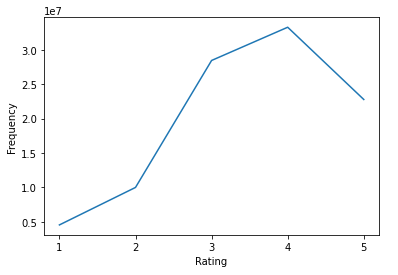
\includegraphics[width=0.5\textwidth]{screenshot20210422222105.png}
	\caption{Frequency of ratings}
\end{figure}

\begin{figure}
	\label{fig:user-rating-freq}
	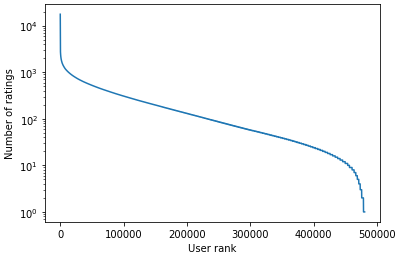
\includegraphics[width=0.5\textwidth]{screenshot20210422222340.png}
	\caption{Number of ratings per user}
\end{figure}

\begin{figure}
	\label{fig:movie-rating-freq}
	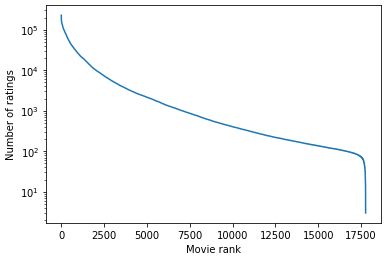
\includegraphics[width=0.5\textwidth]{screenshot20210422223229.png}
	\caption{Number of ratings per movie}
\end{figure}

\subsubsection{Evaluation process}
To evaluate performance, 1425333 rows (about 1.42\% of all data) are speified as the standard "probe".
We perform analysis in the following procedure:

\begin{enumerate}
	\item Train the model with the 99055174 non-probe rows.
	\item Predict user ratings with the 1425333 probe rows.
	\item Compute the \ac{RMSE} between the predicted data and actual data.
\end{enumerate}

In this project, we evaluate three models, namely:

\begin{itemize}
	\item \ac{KNN}, a simple neighbourhood model
	\item \ac{SVD}, a latent factor model that accounts for user bias
	\item \ac{NCF}, a latent factor model that represents features with neural network weights
\end{itemize}

\section{Conclusion}

\subsection{\ac{KNN} model}

\subsection{\ac{SVD} model}

\subsection{\ac{NCF} model}

{\small
	\bibliographystyle{ieee_fullname}
	\bibliography{egbib}
}

\end{document}
